\end{multicols}
\newpage
\section{Sonstiges}
\begin{multicols}{2}

In diese Abschnitt %sollt ihr noch einmal zum Nachdenken angeregt werden,
bekommt eine "Ubersicht "uber das Semesterticket, Hinweise zu einer
anstehenden Exkursion, das Impressum, weitere Ansprechpartner neben der Fachgruppe, Campuskarten und euren Stundenplan.
 
\begin{multicols}{2}
\subsection{Semesterticket}
	Euer Studentenausweis berechtigt euch zur Fahrt auf vielen Zugstrecken in Niedersachsen. Unten seht ihr den Gültigkeitsbereich des Semestertickets im Großraum Hannover. Nach Norden und und Westen deckt das Semesterticket weitere Strecken ab. Einen grober Überblick gibt die nebenstehende Karte. 

	Es dürfen nur Regionalexpress (RE) und Regionalbahn (RB) der Deutschen Bahn AG, sowie teilweise der Metronom in der zweiten Klasse benutzt werden. Also NICHT Strecken der Nordwestbahn (NWB). Einen genauen Überblick findet ihr in Form einer Streckenliste auf der Seite \pageref{streckenliste1}.

	Mehr Details könnt ihr den Seiten des AStA unter \url{http://www.asta.tu-bs.de/semesterticket.php} bzw. \url{http://tinyurl.com/3gn8fhg} entnehmen.
\end{multicols}
\newpage
%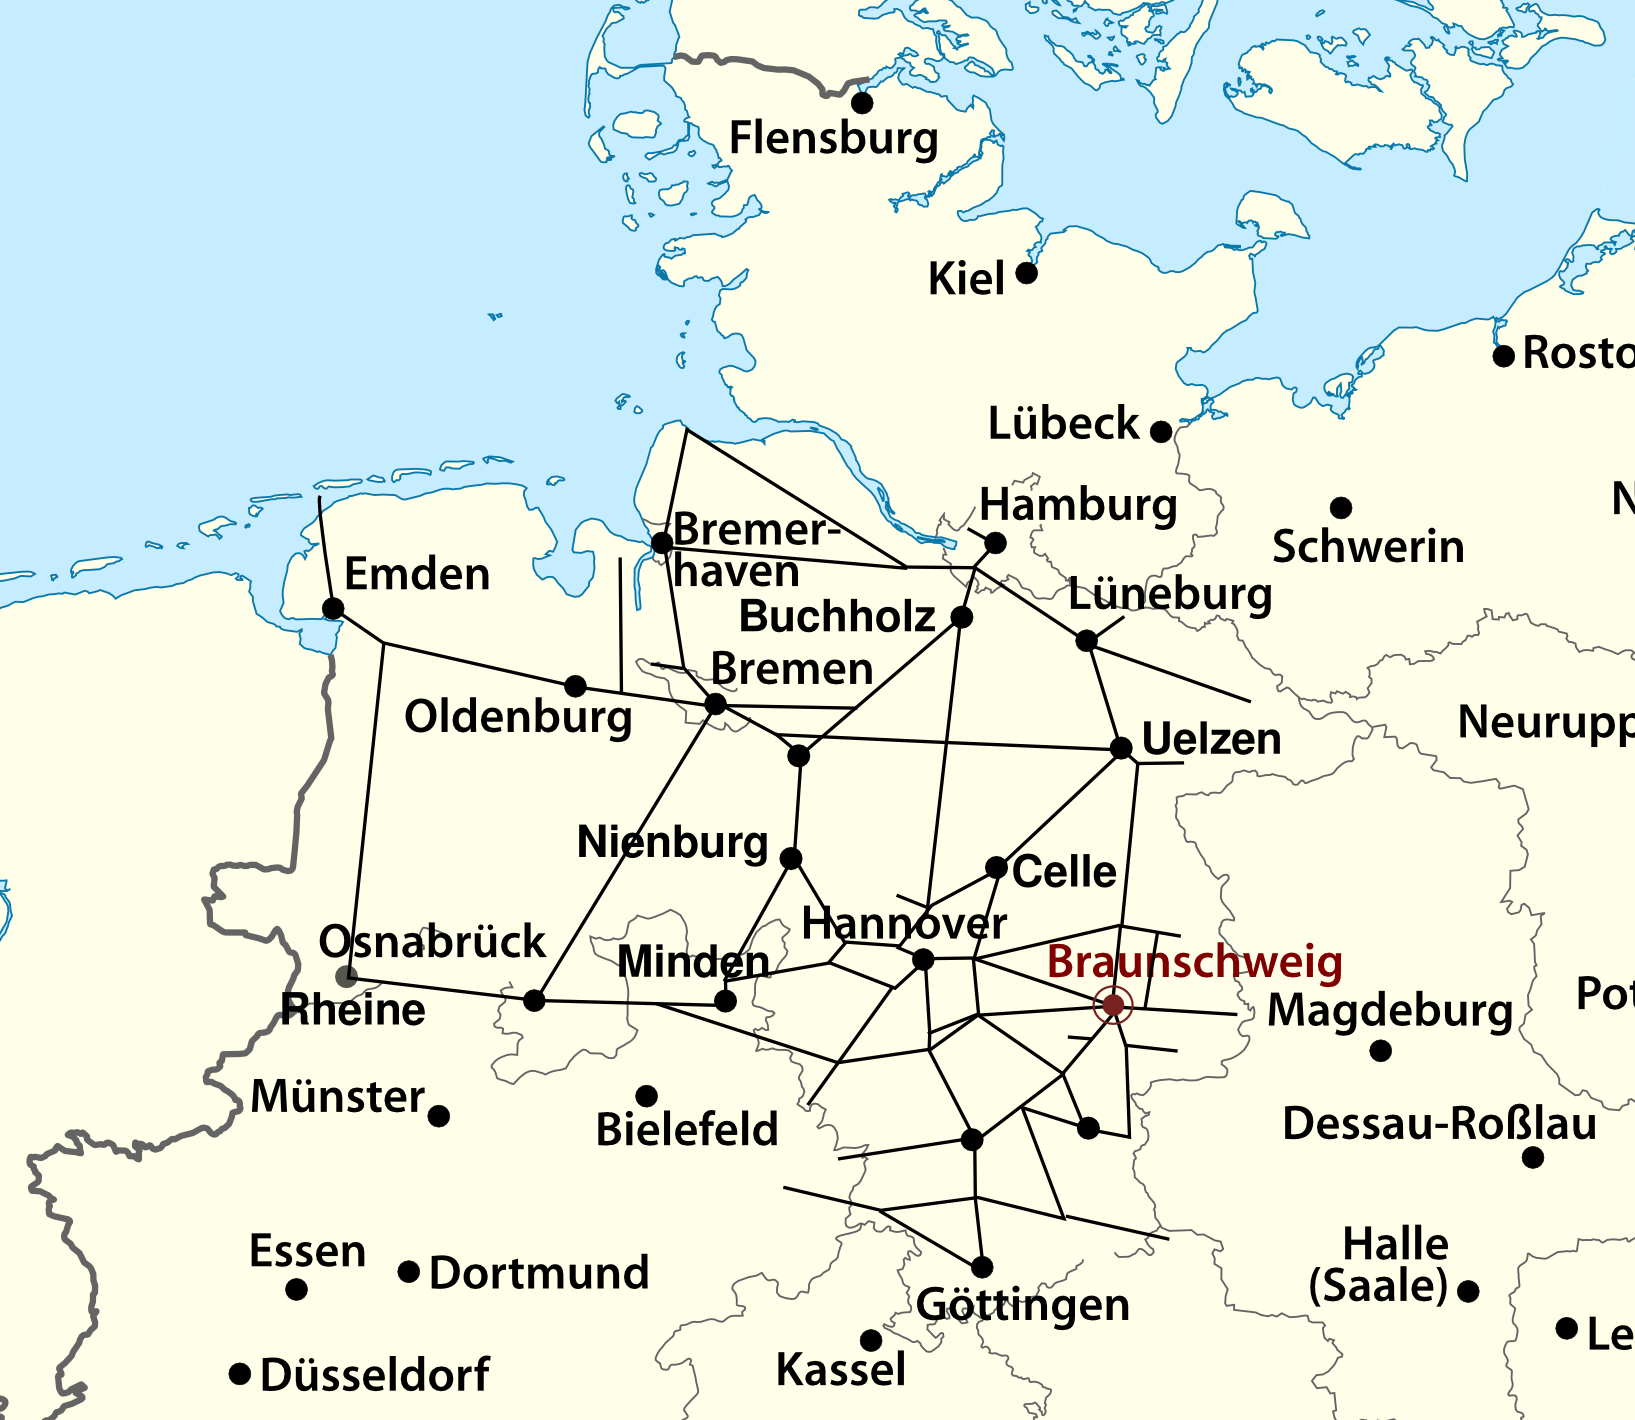
\includegraphics[width=\columnwidth]{bilder/ticket_deutschland.png}
\newpage
%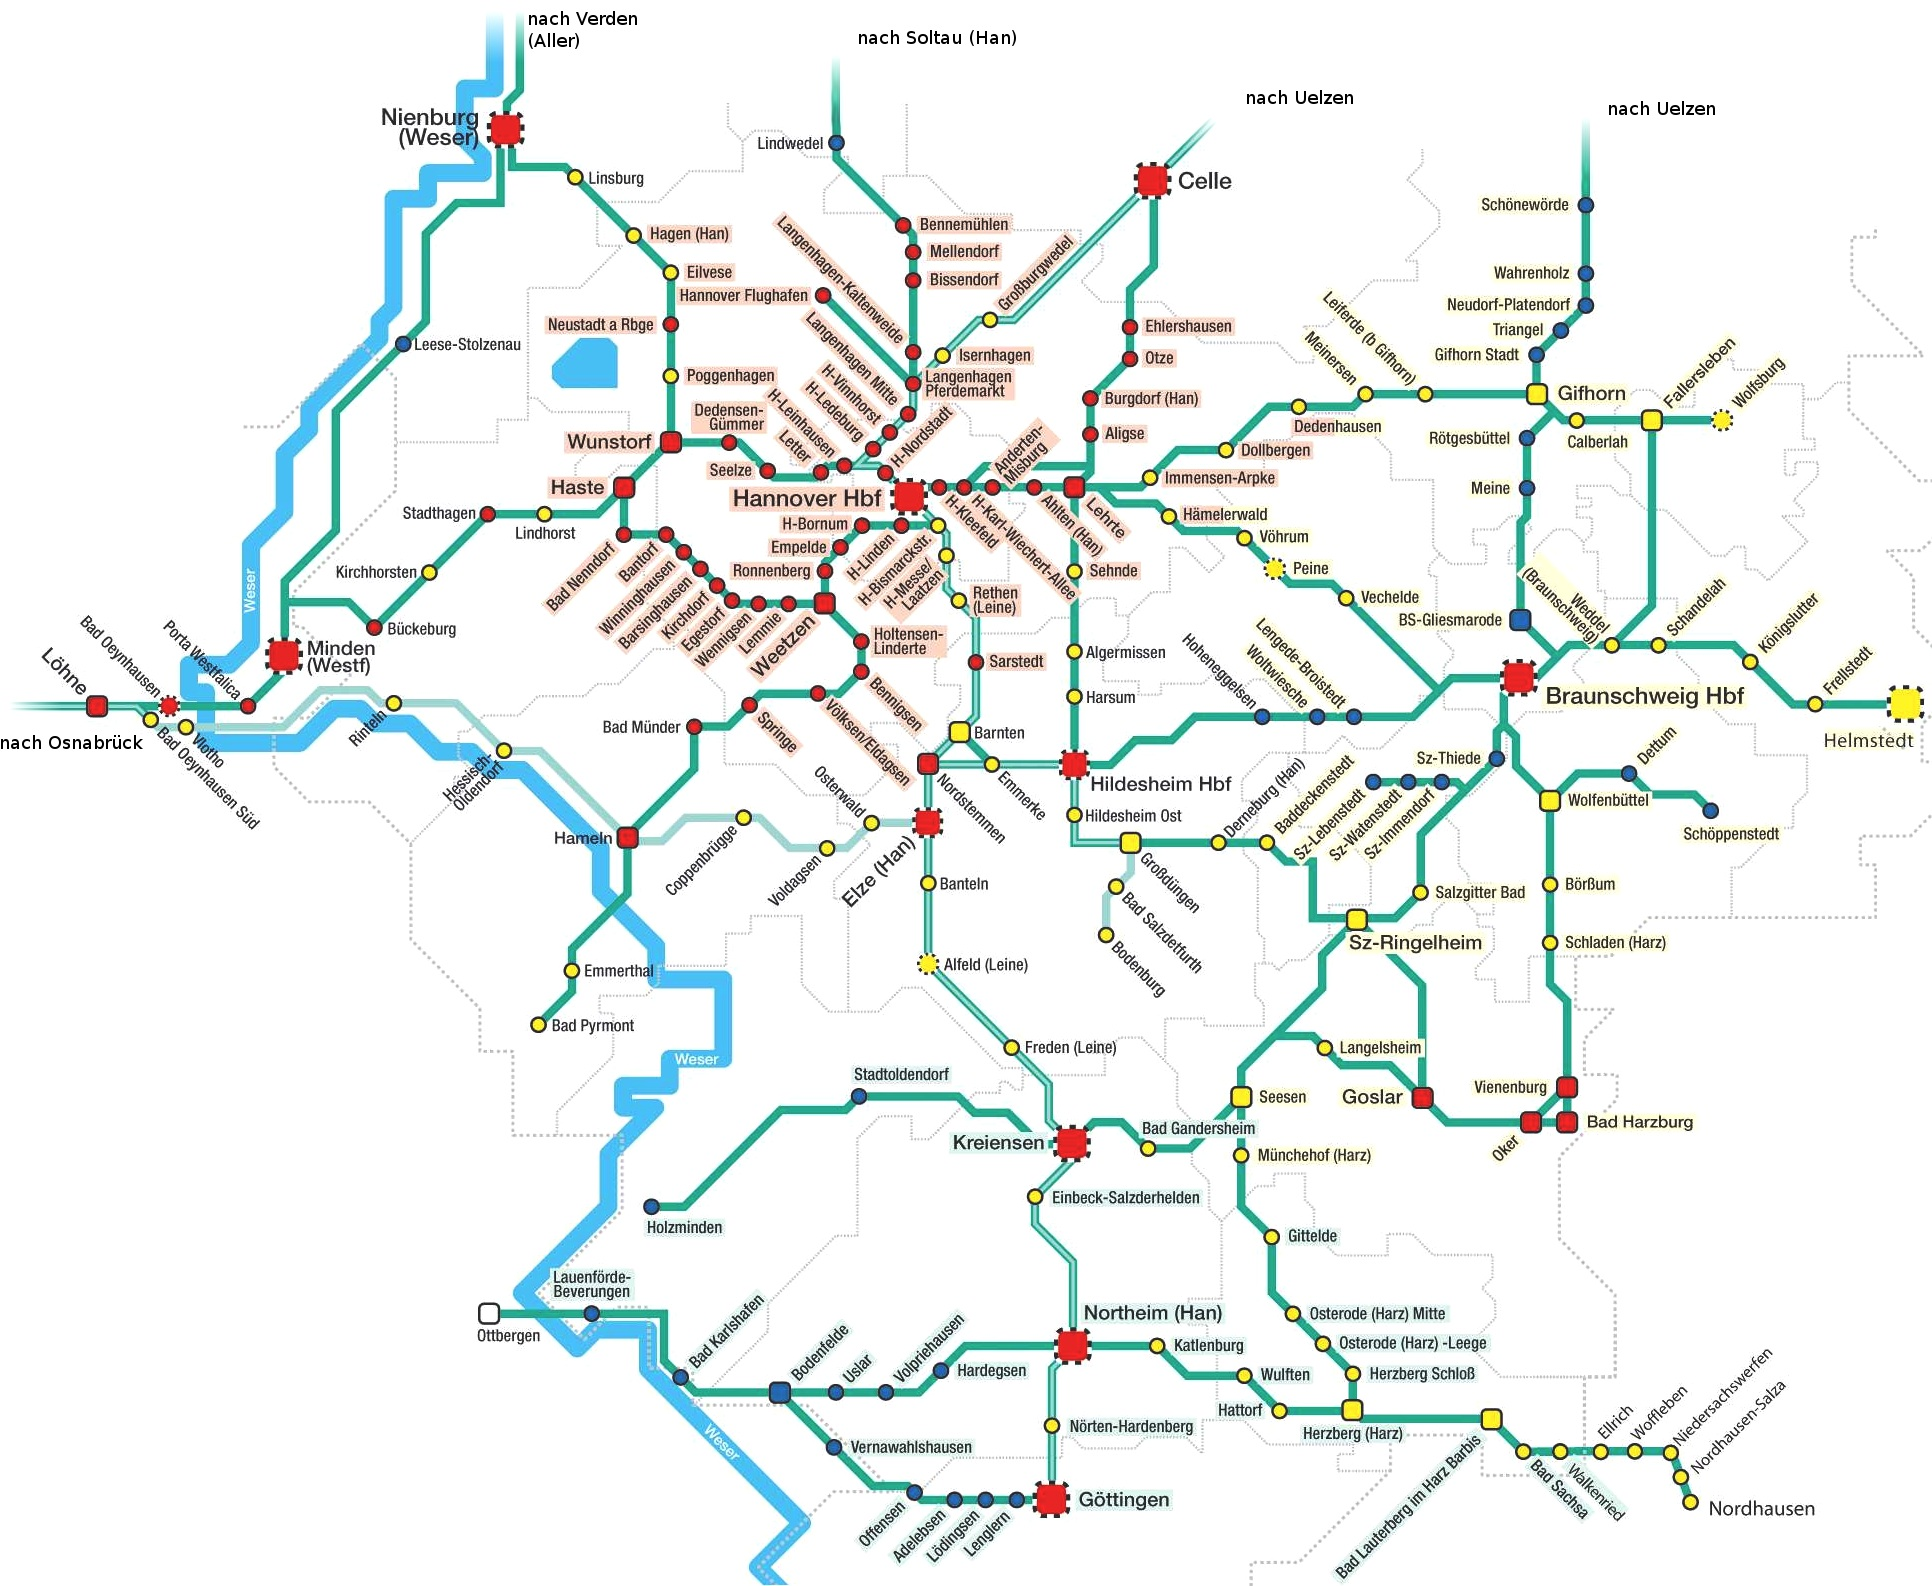
\includegraphics[width=\textwidth]{bilder/ticket_bis_11_Dezember.jpg}
\newpage
\newpage
\begin{multicols}{2}
\subsubsection*{Streckenübersicht Wintersemester 2010/2011 und Sommersemester 2011 gültig ab 1.10.2010}
\label{streckenliste1}
\begin{tabular}{|l|l|l|p{2cm}|}
\hline
\multicolumn{3}{|l|}{\textbf{Strecke/ Streckenabschnitt}}& \textbf{KbN}\\
\textbf{\textit{von}} & \textit{über} & \textbf{\textit{bis}} & \\ \cline{ 1- 4}
Lüneburg &  & Dannenberg Ost & 112 \\ \hline
Braunschweig Hbf & Gifhorn & Uelzen & 115 \\ \hline
Bremen Hbf & Soltau & Uelzen & 116 \\ \hline
Hamburg-Harburg &  & Stade & 121 \\ \hline
Buchholz (Nordheide) & Soltau & Bennemühlen & 123 \\ \hline
Minden Westf. & Nienburg & Rotenburg/Bremen Hbf & 124 \\ \hline
Bremen Hbf &  & Cuxhaven & 125 \footnotemark[1] \\ \hline
Bremen Hbf &  & Bremen-Vegesack & 126 \footnotemark[1] \\ \hline
Echem &  & Lüneburg & 145 \\ \hline
Hannover Hbf & Gifhorn & Wolfsburg Hbf & 300 \\ \hline
Braunschweig Hbf &  & Wolfsburg Hbf & 301 \\ \hline
Uelzen &  & Schnega & 305 \\ \hline
Hannover Hbf & Braunschweig Hbf & Helmstedt & 310 \\ \hline
Braunschweig Hbf & Wolfenbüttel & Schöppenstedt & 312 \footnotemark[2] \\ \hline
Braunschweig Hbf &  & Hildesheim Hbf & 313 \\ \hline
Hannover Hbf & Hildesheim Hbf/Goslar & Bad Harzburg & 320 \\ \hline
Braunschweig Hbf &  & Sz-Lebenstedt & 352 \\ \hline
Braunschweig Hbf & Wolfenbüttel/Vienenburg & Goslar & 353 \\ \hline
Holzminden & Kreiensen & Bad Harzburg & 354 \\ \hline
Ottbergen & Bodenfelde & Göttingen & 356.1 \\ \hline
Ottbergen & Bodenfelde & Northeim & 356.2 \\ \hline
Göttingen & Northeim & Walkenried & 357 \footnotemark[1] \\ \hline
Braunschweig Hbf & Seesen & Herzberg (Harz) & 358 \\ \hline
Haste & Hannover Hbf/Haste & Minden (Westf) & 360.1 \\ \hline
Nienburg (Weser) & Hannover Hbf & Haste & 360.2 \\ \hline
Hannover Hbf & Lehrte & Hildesheim Hbf & 360.3 \\ \hline
Bennemühlen & Hann./Sarstedt & Hildesheim Hbf & 360.4 \\ \hline
Bad Pyrmont & Hameln/Weetzen & Hannover-Flughafen & 360.5 \\ \hline
Celle & Lehrte & Hannover Hbf & 360.6.7 \\ \hline
Hannover Hbf &  & Hannover Bismarckstr. & 361 \footnotemark[1] \\ \hline
Hannover Hbf &  & Löhne (Westf.) & 370 \\ \hline
Löhne (Westf.) & Hameln & Hildesheim Hbf & 372 \\ \hline
Hildesheim Hbf &  & Bodenburg & 373 \\ \hline
Salzbergen & Osnabrück Hbf & Minden (Westf.) & 375 \footnotemark[1] \\ \hline
Bremen Hbf &  & Hannover Hbf & 380 \\ \hline
Osnabrück Hbf &  & Bremen Hbf & 385 \footnotemark[1] \\ \hline
Norddeich Mole & Oldenburg (Oldb) & Bremen Hbf & 390 \footnotemark[1] \\ \hline
Norddeich Mole & Meppen & Rheine & 395 \footnotemark[1] \\ \hline
Emden Hbf &  & Emden Außenhafen & 396 \\ \hline
Leer (Ostfr.) &  & Weener & 397 \\ \hline
\end{tabular}

\footnotetext[1]{nur in den Zügen der DB Regio AG, also nicht in Zügen der Nordwestbahn}
\footnotetext[2]{gültig auch in Bus von  Schöppenstedt-Schöningen-Helmstedt}
\end{multicols}

%\newpage \
\subsection{Lernräume}
	Hier wollen wir euch eine aktuelle Übersicht über Lernräume an der TU Braunschweig geben. Die Liste ist im Moment nicht vollständig. Auf unserem Blog pflegen wir eine Liste, die wir immer dann erweitern, wenn wir einen neuen Lernraum finden.
Wenn du im Laufe deines Studiums einen guten Ort findest, kannst du uns den Raum mitteilen, wir überprüfen das und nehmen ihn dann in die Liste auf.. Alle Gebäude stehen, wenn nicht anders in Anlage 1 der Hausordnung der TU Braunschweig erwähnt, von 7:30 bis 19:30 Uhr offen.
	\subsubsection*{Informatikzentrum}
		\begin{tabular}{|p{4cm}|p{5cm}|p{8cm}|}
			\hline Raum & Öffnungszeiten & Ausstattung \\ 
			\hline Plaza des Informatikzentrums & normal &  Tische und Stühle, Steckdosen unter Bodenabdeckungen zu finden \\
			\hline Fachgruppenraum der Informatik IZ 150 &
			nach Absprache mit Mitgliedern des
			Fachgruppenrates (wir ;) ) & Kaffemaschine,
			Sofas, Tische, WLAN, Steckdosen in Massen sowie Ethernetkabel\\ 
			\hline Fachgruppenraum der Wirtschaftsinformatik
			IZ 159 & nach Absprache mit Mitgliedern des
			Fachgruppenrates Wirtschaftsinformatik & Sofas, Tische, WLAN und Steckdosen \\ 
			\hline CIP Pool IZ G40 & normal & Rechner-Pool mit Linux-PCs, Tafel\\ 
			\hline Gruppenarbeitsraum IZ 033 & 
			
			Solange nicht anders belegt. Den Schlüssel
			erhält man gegen Pfand im Seketariat der Robotik bei Frau Engel,
			Raum G13.
			 &
			Tische, Stühle, WLAN
			\\
			\hline
		\end{tabular}
	\subsubsection*{Andere Lernräume}
		\begin{tabular}{|p{4cm}|p{5cm}|p{3.6cm}|p{4cm}|}
 			\hline Raum & Öffnungszeiten & Ausstattung & Anmerkung  \\  
			\hline Grotrian  Zimmerstraße 24 & Normal  &
			Alte Tische und Stühle, WLAN, vereinzelt Tafeln & Wenn Mitglieder der verschiedenen Fachgruppen anwesend sind hat das Grotrian meist länger offen. Da dies oft der Fall ist kann man hier meist lange lernen. \\ 
			\hline Bibliothek & Mo - Fr: 07:00 - 24:00 Sa:
			10:00 - 20:00& Niedrige Tische und Stühle,
			Ruhezone, WLAN, Rechnerarbeits\-plätze, Kopierer &  nicht zum  Lernen in der Gruppe  geeignet \\ 
			\hline Mensa / Cafeteria & Mo -Do: 08 - 20:00 Uhr Fr: 08:00 - 15:00 & Tische, Stühle, kein (!) WLAN, einzelner Rechner mit Netzzugang, Verpflegung incl. Selbstbedienungs-Kaffeeautomat& Probleme: Nicht durchgehend geöffnet, die Plätze sind primär zu Essen gedacht, von Lernsessions zu den Stoßzeiten sollte man also im eigenen und fremden Interesse absehen. \\ 
			\hline Bei dir zuhause & immer & Deine Sache & Achtung: Ablenkung ;) \\ 
			\hline Das eine oder andere Cafe / Kneipe & kommt drauf an & wechselhaft &Siehe die beiden vorherigen \\
			\hline
		\end{tabular}

\begin{multicols}{2}
% !TEX root = ../../1-te.tex

\subsection{Ansprechpartner}

	\paragraph{Fachgruppenrat}
		Im Normalfall treffen wir uns jede Woche zum Fachgruppentreffen im Raum 149/150 des Informatikzentrums. Den  Termin findest du auf unserem Blog \fginfoUrl. Falls du eine Frage hast, kannst du gerne zum regulären Fachgruppentreffen kommen, oder einfach so mal vorbei schauen, ob jemand da ist. Gerade im Semester sind die Chancen gut, einen von uns anzutreffen ;)
		\\
		\\
		Tipp: In der Stunde vor dem Treffen füllt sich der Raum schon langsam, also hast du da gute Chancen, Probleme in kleinerer Runde zu besprechen. Ansonsten erreichst du uns natürlich via Email unter \verHref{6}{mailto:fginfo@tu-bs.de}{fginfo@tu-bs.de}. 

	\paragraph{Fachspezifisches}
		Bei Fragen zu einem speziellen Fach wendest du dich am
		besten an den oder die Professor/in bzw. Dozent/in -
		keine/r von denen beißt! Am besten findest du sie über die Seiten der jeweiligen Institute 
		oder über die Personensuche unter \verUrl{6}{http://www.tu-braunschweig.de/suchoptionen/personen}.

	\paragraph{Studiengangskoordinatorin}
		Yvonne Sehnert \\
		Sie steht bereit, um deine Fragen zu beantworten, und für alles, was sie nicht selbst weiß, weiß sie, an wen sie die Frage weiterleiten muss.\\
		Carl-Friedrich-Gauß-Fakultät\\
		Rebenring 58 A | Raum 124\\
		Sprechzeiten: Nach  Vereinbarung\\
		Telefon: (0531) 391-2843\\
		E-Mail: \verHref{6}{mailto:informatik-studium@tu-bs.de}{informatik-studium@tu-bs.de}

	\paragraph{Prüfungsamt}
		Rebecca Weidner\\
		Carl-Friedrich-Gauß-Fakultät\\
		Rebenring 58 A | Raum 127\\
		Tel.: (0531) 391-2844\\
		Fax: (0531) 391-8220\\
		E-Mail: \verHref{6}{mailto:pa-informatik@tu-braunschweig.de}{pa-informatik@tu-braunschweig.de}\\
		Sprechzeit im Semester:\\
		Di. und Do.: 10:00–12:00 Uhr und 14:00-16:00 Uhr\\
		Sprechzeit in der vorlesungsfreien Zeit:\\
		Di. und Do. 10:00-12:00 Uhr

\end{multicols}
\begin{multicols}{2}

\subsection{Campuskarte}
\label{campuskarte}
Bereits auf Seite \pageref{plan} habt ihr einen einfachen Campusplan
gesehen. Es gibt aber noch diverse andere Online:\\
Eine aktuelle Campuskarte, die durchsucht werden kann findet sich im
TUgether Portal unter \nurl{https://tugether.tu-braunschweig.de/}. Du
kannst dich dort mit deiner Y-Nummer einloggen.\\\\

Ein Raumplan für das 1. und 2. OG des Informatikzentrums findet sich
unter\\ \nurl{http://www.ibr.cs.tu-bs.de/rooms/rooms.html}
Sollten euch die genannten Links zu unhandlich zum Abtippen sein, findet ihr
auch alle unter
\nurl{http://fginfo.cs.tu-bs.de/index.php/studium/lernraume/}.
Dort findet ihr auch virtuelle Campustouren, die  in einem Web 2.0 Seminar entstanden und
bei Google Maps gehostet sind.
%ekeliger tabellenhack NICHT NACHMACHEN
%\begin{tabular}{c}
%\\  \\ \\ \\ \\ \\
%\end{tabular}
\subsection{Exkursion zum 27C3}
Die Fachgruppe plant eine Exkursion zum 27C3. \\Dabei handelt es sich um
die diesjährige Ausgabe des Chaos Communication Congress des Chaos
Computer Clubs.\\ Die Exkursion wird aus
Studiengebühren finanziert und befindet sich derzeit noch in der
Planungsphase. \\Mehr Informationen findet ihr auf folgenden
Webseiten:\\
\nurl{http://events.ccc.de/congress/}\\
\nurl{http://fginfo.cs.tu-bs.de/index.php/tag/27c3/}\end{multicols}
% !TEX root = ../1-te.tex

\begin{description}
\item[Herausgeber:]
	Fachgruppe Informatik\\
	c/o AStA der TU Braunschweig\\
	Katharinenstraße 1\\
	38106 Braunschweig\\
	Tel.: 0531/391-4569\\
	E-Mail: \verHref{5}{mailto:fginfo@tu-bs.de}{fginfo@tu-bs.de}\\
	Webseite: \fginfoUrl
\tocheck{4}{Mitglieder das FG-Rats nennen}
\item[Cover:] Sophia Scholtka und Rebecca Finster
\item[Comics:] Randall Munroe -- XKCD (\verUrl{5}{http://xkcd.com/})
\end{description}

 %\newpage
%\nurl{http://maps.google.de/maps/ms?ie=UTF8&hl=de&msa=0&msid=110022173347618328583.00044f5213e3e4ab36c53&z=17}%\begin{multicols}{2}
%\hfill%\end{multicols}
%\begin{multicols}{2}
%Hier fehlt noch Text, Ein Raumplan für das 1. und 2. OG des Informatikzentrums findet sich unter http://www.ibr.cs.tu-bs.de/rooms/rooms.htmlden man aber einfach von der fg-Seite nehmen kann. Insbesondere geht's da um die Verweise auf die diversen Online-Karten wie er unter \url{http://fginfo.cs.tu-bs.de/index.php/studium/lernraume/} steht.

% Dieser Trick hilft uns, eine neue Seite zu erzwingen
% (auf diese passt eh nix sinnvolles mehr) und dennoch die 
% Spaltenlängen auszubalancieren.
%Hier fehlt noch Text, den man aber einfach von der fg-Seite
%nehmhttp://events.ccc.de/congress/en könnte, wenn denn dort mal was
%stünde.
%\end{multicols}
\newpage
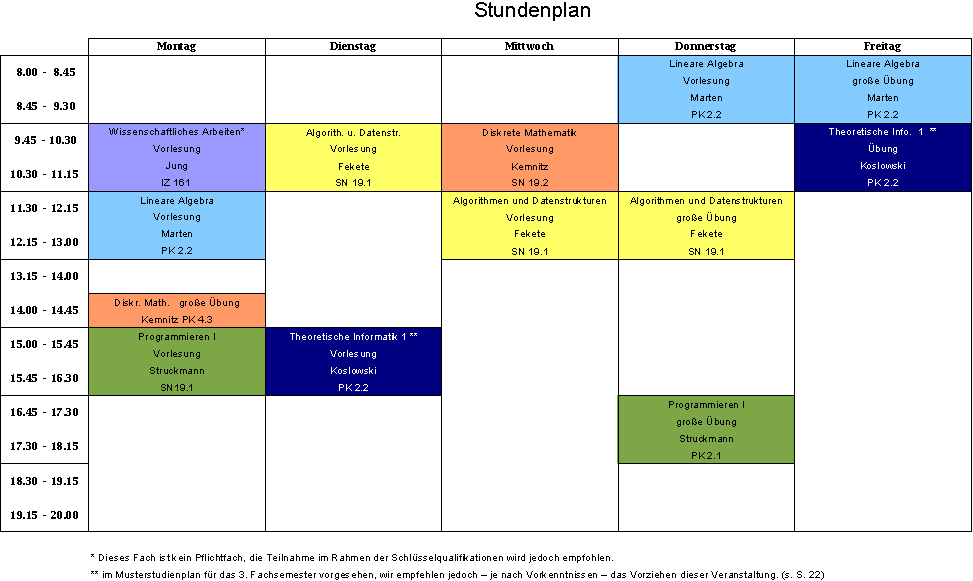
\includegraphics[angle=90,totalheight=\textheight, width=1.25\textwidth]
{texte/nuetzliches/stundenplan}

%%% Local Variables: 
%%% mode: latex
%%% TeX-master: "../../1-te"
%%% End: 
